\setcounter{mtc}{4} %indique le numero reel du chapitre, pour la mini Table of Contents
\chapter{Présentation de l’entreprise}
\minitoc  %insert la minitoc

\graphicspath{{Chapter1/figures/}}
%==============================================================================
\pagestyle{fancy}
\fancyhf{}
\fancyhead[R]{\bfseries\rightmark}
\fancyfoot[R]{\thepage}
\renewcommand{\headrulewidth}{0.5pt}
\renewcommand{\footrulewidth}{0pt}
\renewcommand{\chaptermark}[1]{\markboth{\MakeUppercase{\chaptername~\thechapter. #1 }}{}}
\renewcommand{\sectionmark}[1]{\markright{\thechapter.\thesection~ #1}}

\begin{spacing}{1.2}
%==============================================================================

\section*{Introduction}
Le groupe \textbf{Délice} est un groupe tunisien de l’industrie agroalimentaire qui opère essentiellement dans l’industrie laitière.\newline


C’est en 1978, que Mr. Hamdi MEDDEB fonde sa première entreprise, la Société Tunisienne des Industries Alimentaires (STIAL), avec l’aide du fond de promotion et de décentralisation industrielle. Spécialisée dans le yaourt et les dérivés laitiers, elle devient peu à peu un leader de l’industrie laitière en Tunisie, avec 30\% des parts de marché en 1993.\newline


Avec la fondation de la Centrale laitière du Cap-Bon, spécialisée dans la fabrication, le conditionnement et la commercialisation du lait et de ses dérivés, et la Société de Commerce et de Gestion (SOCOGES), chargée de la distribution, le noyau du groupe Délice est constitué, suscitant ainsi l’intérêt de la multinationale \textbf{Danone}.\newline


En 1997, un partenariat stratégique entre le Groupe Délice et Danone a été concrétisé à travers la cession de 50 \% du capital des sociétés STIAL et SOCOGES à la Compagnie Gervais Danone `CGD'.\newline

\section{Fiche technique de STIAL Délice Danone}

\begin{table}[!h]
	\centering
	\caption{Fiche signalétique de STIAL Délice Danone}
	\footnotesize
	\begin{tabularx}
	{\linewidth}{
  |>{\centering{}\vspace*{\fill}}X
  |>{\vspace*{\fill}}X
  <{\centering{}}|}
			\hline
\textbf{Raison Sociale}			&	Société Tunisienne des Industries Alimentaires laitière (STIAL) \\
			\hline
\textbf{Statut Juridique}			&	Société Anonyme \\
  			\hline
\textbf{Catégorie}			&	Société privée locale \\
			\hline
\textbf{Siège social}			&	Immeuble le DÔME, Rue de lac Léman, Les berges du lac 1053, Tunis \\
			\hline
\textbf{Adresse}			&	Km 1, Route de Menzel Bouzelfa – 8020 SOLIMAN \\
			\hline
\textbf{Téléphone}			&	(+216) 70 024 200 \\
			\hline
\textbf{Fax}			&	(+216) 72 291 153 \\
			\hline
\textbf{Date de création}			&	14 décembre 1978 \\
			\hline
      \textbf{Président directeur général}			&	Mr Hamdi MEDDEB \\
      			\hline
            \textbf{Effectif}			&	1400 personnes \\
            			\hline
                  \textbf{Site We}			&	 http://www.delice.tn \\
                  			\hline
                        \textbf{secteur d’Activité}			&	Produits Laitiers \\
                        			\hline
                              \textbf{Chiffre d’affaires}			&	600 MDT \\
                              			\hline
	\end{tabularx}
	\label{tab:usecasediagram}
\end{table}


\section{Produits commercialisés}
Les produits de Délice Danone se classent parmi les plus qualifiés sur le marché local Tunisien .\newline

La large gamme des produits laitiers fabriqués par la société comprend :


\begin{table}[!h]
	\centering
	\caption{Liste de produits fabriqués par  Délice Danone }
	\footnotesize
	\begin{tabularx}
	{\linewidth}{
  |>{\centering{}\vspace*{\fill}}X
  |>{\vspace*{\fill}}X
  <{\centering{}}|}
			\hline
\textbf{Les produits fermentés}			&	\textbf{Les produits non fermentés} \\
			\hline
Yaourt étuvé nature


 Yaourt étuvé aromatisé


 Yaourt Brassé aromatisé


 Brassé fruits


 Activia nature


 Activia nature 0\%


 Activia aromatisé ferme


 Yaourt à boire


 Fromage : Danino et jockey
 		& Crèmes desserts : Danette


    Boissons lactées : DANAO \\
                              			\hline
	\end{tabularx}
	\label{tab:produit}
\end{table}
\newpage
\section{Organigramme de STIAL Délice Danone}

\begin{figure}[!ht]\centering
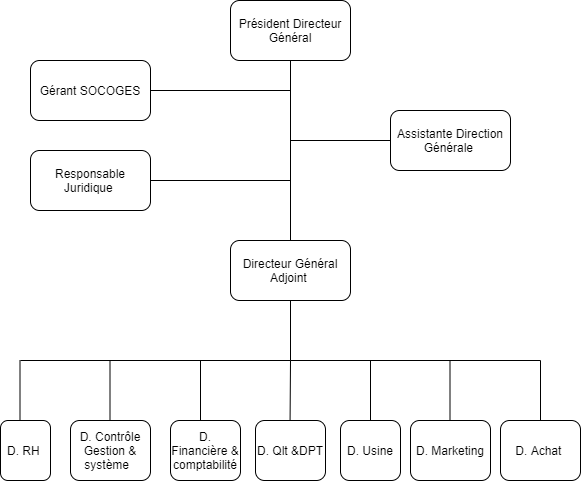
\includegraphics[scale=0.7]{organigramme.png}
\caption{Organigramme de STIAL Délice Danone}
\label{fig:fig1}
\end{figure}
\section{La politique qualité et sécurité des aliments  de  STIAL Délice Danone}
Dans sa politique qualité, Délice Danone a formalisé les engagements suivant :
\begin{itemize}

\item Viser l'excellence de la qualité \& sécurité des ses produits
\item Développer la qualité nutritionnelle de ses produits
\item Améliorer la qualité des matières premières
\item Améliorer la qualité de la distribution de ses produits
\item Développer les compétences qualité de ses collaborateurs
\item Développer la culture qualité au sein de l’entreprise
\end{itemize}

\section{ Les certifications acquises }
 STIAL Délice Danone ne cesse de développer sa démarche qualité et ceci se traduit par les différentes certifications :

 \begin{itemize}

 \item Certification selon ISO 22 000 (version 2005) : 2011

 \item Certification selon FSSC 22 000 (version 4.1) : 2018

 \item Certification selon FSSC 22 000 (version 5) : Juin 2020
 \end{itemize}
 \section{Les réalisations en matière de satisfactions des clients }
 STIAL Délice Danone assure en permanence l’écoute de ses clients en vue d'accroître leur satisfaction.


Les enquêtes annuelles de satisfaction des clients  dépassent les 90\%.


Les enquêtes mensuelles de satisfaction des grandes surfaces qui dépassent les 90\%.


Les prospections et visites clients et détaillants.


La conception d’un site web interactif.

\section{STIAL Délice Danone et l’environnement}
Mise en place d’une station de prétraitement des eaux usées en
Gestion des déchets solides :


Réduction de la consommation d’eau de et de l’électricité de


Réduction des émissions gazeuses par l’utilisation du gaz naturel à la place du fuel

\section{Diagramme de  production}
La figure 2  montre les principales étapes de production du yaourt  dans l’usine depuis la réception du lait jusqu'à l’expédition des produits finis.

\begin{figure}[!ht]\centering
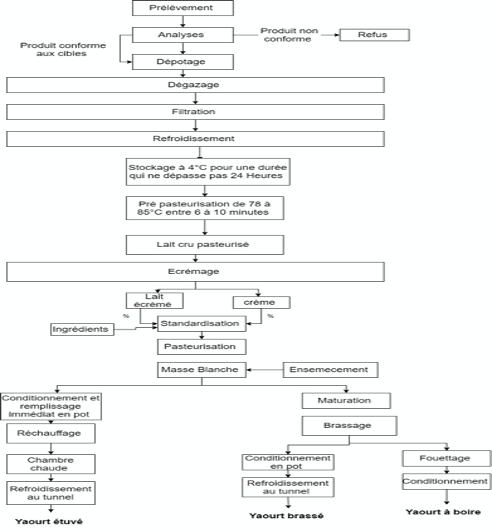
\includegraphics[scale=0.9]{fabrication_yaourt.png}
\caption{Diagramme général de fabrication du yaourt (selon Délice Danone)}
\label{fig:fig1}
\end{figure}




%==============================================================================
\end{spacing}
